\part{Connection}
\label{connection}

Vlastní protokol je rozdělen do dvou vzájemně nezávislých vrstev. To umožňuje oddělení funkcionality aplikačního síťového protokolu, přes který se posílají data, a vlastní datové struktury. Na obrázku \ref{connection.pictures.protocol_layers} jsou ilustrovány vrstvy protokolu.

\begin{figure}[h]
  \centering
  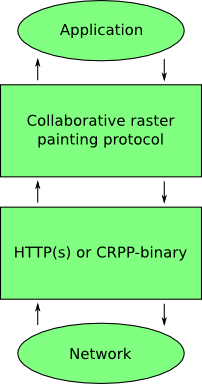
\includegraphics[width=0.30\textwidth]{diagrams/protocol_layers.png}
  \caption{Protocol layers diagram}
  \label{connection.pictures.protocol_layers}
\end{figure}

Vrchní vrstva předává spodní vrstvě monolitické bloky dat, které spodní vrstva dopraví vrchní vrstvě na druhé straně spojení. Vrchní vrstva je popsána v části \ref{up_layer} a spodní v části \ref{down_layer};

\chapter{Data types}
\label{connection.data_types}

Pokud není uvedeno jinak, tak všechny celočíselné hodnoty jsou bezeznaménkové.

\section{Unsigned integers}
\label{connection.data_types.unsigned_integer}

Každý bit s hodnotou $1$ reprezentuje číslo $2^{p}$. Kde $p$ je pozice bitu (poslední bit -- v textu nejpravější -- posloupnosti má pozici $0$). Bity s hodnotou $0$ jsou rovny $0$. Rovnice \ref{equation.unsigned-integers-sum} udává hodnotu čísla.

\begin{equation}
\label{connection.equations.unsigned_integer}
\sum_{p = 0}^{n - 1} b_p 2^p
\end{equation}

kde $p$ je pozice bitu (poslední ma hodnotu $0$, pak roste směrem k předcházejícím), $n$ je celkový počet bitů reprezentujících číslo, $b_p$ je hodnota bitu ($0$ nebo $1$) na pozici $p$.

Například posloupnost $00001010$ má hodnotu $10$ ($2^1 + 2^3$).

\section{Signed integers}

Hodnota znaménkového celého čísla je součet čísel $a$ a $b$ (tedy ${value} = a + b$). 

Hodnotu proměnné $a$ uručje vzorec $a = -2^{n - 1} \cdot f$, kde $n$ je počet bitů reprezentujících číslo a $f$ první bit ($0$ or $1$).

Hodnotu promměné $b$ určuje vzorec \ref{connection.equations.unsigned_integer} přičemž první bit není do vzorce vložen. Například posloupnost $10011$ by měla hodnotu $b = 2^0 + 2^1$ (není zahrnut první bit $1$).

Příklad: číslo reprezentované bity $1011$ má hodnotu $-5$ ($a = -2^3 \cdot 1 = -8$, $b = 2^1 + 2^0 = 3$, $a + b = -8 + 3 = -5$).

\section{Floating point numbers}

Reálná čísla jsou reprezentována podle standardu IEEE 754 ve 32 bitech.

\section{Logical value (booleans)} 

Logické hodnoty (boolean) jsou reprezentovány jedním bytem, kde samé nuly ($00000000$) reprezentují hodnotu \emph{false} a hodnota jedna ($00000001$) reprezentuje hodnotu \emph{true}. Ostatní hodnoty jsou považovány za nevalidní.

\section{Strings}

Veškerý text (řetězce zanků) je kódován jako UTF-8. V některých případech jako posloupnost ASCII znaků, to je ovšem vždy uvedeno. Všude je rozlišováno mezi malými a velkými písmeny (case sensitive).